\documentclass{beamer}
\usepackage{listings}
\usepackage[english]{babel}
\usepackage[utf8]{inputenc}
\usepackage{subfig}
\usepackage{booktabs}
\usepackage{graphicx,hyperref,ru,url}
\usepackage[smaller]{acronym}
\usepackage[Q=yes]{examplep}
\usepackage{caption}
\lstset{language=bash}          % Set your language (you can change the language for each code-block optionally)
\captionsetup{font=scriptsize,labelfont=scriptsize}
%\usetheme{Copenhagen}
% The title of the presentation:
%  - first a short version which is visible at the bottom of each slide;
%  - second the full title shown on the title slide;
\title[ MitM attacks]{Network Security Lab Activity:\\  Man in the Middle (MitM) attacks}

% Optional: a subtitle to be dispalyed on the title slide
%\subtitle{Show where you're from}

% The author(s) of the presentation:
%  - again first a short version to be displayed at the bottom;
%  - next the full list of authors, which may include contact information;
\author[G. Gemmi, L. Brugnera]{\textbf{Gabriele Gemmi \\ Lorenzo Brugnera}}

% The institute:
%  - to start the name of the university as displayed on the top of each slide
%    this can be adjusted such that you can also create a Dutch version
%  - next the institute information as displayed on the title slide
\institute[]{
  University of Trento}

% Add a date and possibly the name of the event to the slides
%  - again first a short version to be shown at the bottom of each slide
%  - second the full date and event name for the title slide
\date[18/04/2018]{
 Wednesday, 18 April 2018}

\begin{document}

\begin{frame}
  \titlepage
\end{frame}

% \begin{frame}
%   \frametitle{Outline}
%
%   \tableofcontents
% \end{frame}

% Section titles are shown in at the top of the slides with the current section
% highlighted. Note that the number of sections determines the size of the top
% bar, and hence the university name and logo. If you do not add any sections
% they will not be visible.
\section{Introduction}

\begin{frame}
  \frametitle{Outline}
  \begin{itemize}
    \item How to mount a MitM attack
    \begin{itemize}
      \item ARP Spoofing
      \item DHCP (DHCPv6) poisoning
      \item Evil Twin
    \end{itemize}
    \item Attacks that can be mounted after the MitM
    \begin{itemize}
      \item HTTP Interception
      \item SSL Stripping
      \item HSTS Bypass
      \item DNS Spoofing
    \end{itemize}
  \end{itemize}


\end{frame}

\begin{frame}
  \frametitle{What is a MitM attack?}
  \begin{figure}
  \includegraphics[width=0.5\textwidth]{figures/mitm_diagram}
  \caption*{Diagram of a MitM attack}
  \end{figure}
  \only<1>{
    \begin{block}{Requisites}
      \begin{itemize}
        \item The attacker must be near the victim (in the same local network)
      \end{itemize}
    \end{block}
  }
  \only<2>{
  \begin{block}{How to mount this attack}
    \begin{itemize}
      \item The attacker must be physically connected between the victim and the rest of the network
\\      \centering{or}
      \item The attacker must hijack the traffic from the victim to himself
    \end{itemize}
  \end{block}
  }

\end{frame}


\begin{frame}
  \frametitle{Network layer attacks}
  \begin{block}{}
    \begin{itemize}
      \item ARP poisoning
      \item DHCP (DHCPv6) poisoning
      \item Evil Twin
    \end{itemize}
  \end{block}

\end{frame}

\begin{frame}
  \frametitle{ARP Poisoning}
  \begin{block}{How it works}
  \begin{itemize}
    \item The attacker floods the network with poisoned ARP messages
    \item The mapping between IPs and MACs is altered in order to hijack the communication through the attacker
  \end{itemize}
\end{block}
  \begin{figure}
    \includegraphics[height=115px]{figures/arp_spoofing}
    \caption*{ARP Spoofing attack diagram}
  \end{figure}
\end{frame}

\begin{frame}
  \frametitle{ARP Poisoning}
  \begin{block}{How to prevent it?}
  \pause
  \begin{itemize}
    \item ARP poisoning proof switches
    \item VPN
  \end{itemize}
\end{block}
\end{frame}
\begin{frame}
  \frametitle{DHCP (DHCPv6) poisoning}
  \begin{block}{How it works}
  \begin{itemize}
    \item The attacker sets-up a rogue DHCP server
    \item Each time a victim sends a DHCP request the rogue server answers with a forged response
    \item The response contains a malicious default gateway to perform the MitM attack
  \end{itemize}
\end{block}
  \begin{figure}
  \includegraphics[height=95px]{figures/dhcp_poisong}
  \caption*{DHCP poisoning attack diagram}
  \end{figure}
\end{frame}


\begin{frame}
  \frametitle{DHCP (DHCPv6) poisoning}
  \begin{block}{How to prevent it?}
  \pause
  \begin{itemize}
    \item A smart switch can be configured to allow DHCP response only on certain trusted ports
  \end{itemize}
\end{block}
  \begin{figure}
  \includegraphics[height=95px]{figures/dhcp_snooping}
  \caption*{DHCP snooping diagram}
  \end{figure}
\end{frame}


\begin{frame}
  \frametitle{Evil Twin}
  \begin{block}{How it works}
  \begin{itemize}
    \item The attacker sets-up a rogue Wi-Fi Access Point with the same ESSID as the target network
    \item The victim must receive the rogue AP with a stronger signal than the legit one
  \end{itemize}
\end{block}
  \begin{figure}
    \includegraphics[height=110px]{figures/evil-twin}
    \caption*{Evil Twin attack diagram}
  \end{figure}
\end{frame}

\begin{frame}
  \frametitle{Evil Twin}
  \begin{block}{How to prevent it?}
  \pause
  \begin{itemize}
    \item A simple authentication (WPA) doesn't ensure the client that the AP is legit (The attacker just need to discover the key)
    \item The client must authenticate the AP (802.1x) and verify its legitimacy
  \end{itemize}
\end{block}
\end{frame}

\section{Laboratory preparation}
\begin{frame}
\frametitle{Network Topology}
\begin{figure}
  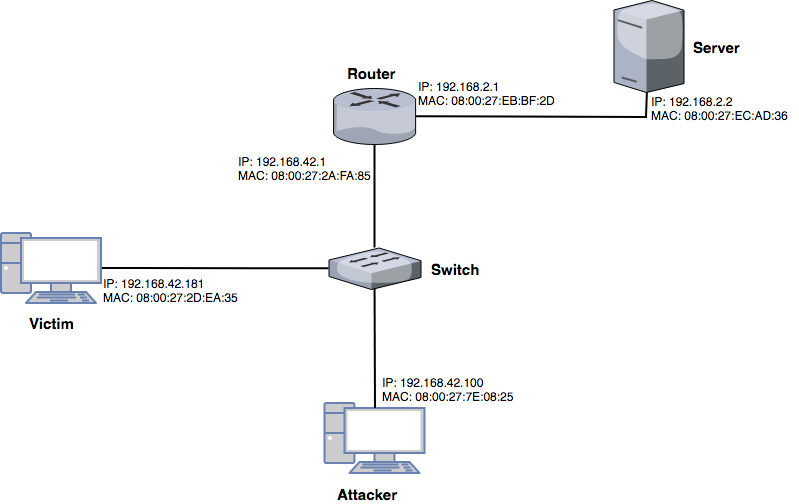
\includegraphics[height=190px]{figures/net_topo}
  \caption*{Topology of the VMs network}
\end{figure}
\end{frame}


\begin{frame}
\frametitle{Tools}
This is a list of tools we will be using in this lab, in the next slides the usage and the purpose will be explained
\vfill
\begin{block}{}
  \begin{itemize}
    \item arpspoof
    \item wireshark
    \item dnsspoof
    \item sslstrip
    \item sslstrip2
    \item dns2proxy
  \end{itemize}
\end{block}

\end{frame}


\begin{frame}
\frametitle{Tips and Tricks}

\begin{block}{Useful infos}
  \begin{itemize}
    \item Type \texttt{sudo} before every command, the password  is ``netsec''
  \end{itemize}
\end{block}
\begin{block}{To do after every exercise}
\begin{itemize}
  \item Flush the DNS cache: \texttt{systemd-resolve --flush-cache}
  \item Clean the iptables chains \texttt{iptables -t <chain name> -F}
\end{itemize}
\end{block}

\end{frame}



\begin{frame}
\frametitle{MitM Network attack}
\begin{block}{}
  \begin{itemize}
    \item To mount the following attacks you can use any of the attacks we illustrated you
    \item Since you already know how to mount it and due to its simplicity, we wll be using ARP spoofing
  \end{itemize}
\end{block}

\begin{block}{}
  \begin{itemize}
    \item You can use either ettercap or this simple command line tool
    \texttt{arpspoof -t <victim ip> -r <router ip>}
  \end{itemize}
\end{block}
\end{frame}


\begin{frame}{How to start the laboratory}
  \begin{block}{}
    \begin{itemize}
      \item Open virtualbox
      \item Run "netsec\_router" and "netsec\_server" in headless mode
      \item Run "netsec\_victim" and "netsec\_malicious" normally
    \end{itemize}
  \end{block}
\end{frame}

\section{Attacks}
\begin{frame}{HTTP Interception}
  \begin{block}{How it works}
    \begin{itemize}
      \item Using wireshark it's possible to capture all the traffic that flows between the victim and the router
      \item Sensitive information can be sniffed by the attacker
    \end{itemize}
  \end{block}
\end{frame}

\begin{frame}{HTTP Interception}
  \begin{block}{Exercise 1}
    \begin{itemize}
      \item Mount an MitM network attack
      \item Open a browser and navigate to ``http://www.homepage.it''
      \item Sniff the HTTP traffic exchanged between the victim and the server
    \end{itemize}
  \end{block}
\end{frame}

\begin{frame}{HTTP Interception}
  \begin{block}{How to prevent?}
  \pause
  \begin{itemize}
    \item An encrypted channel can preserve the confidentiality
    \begin{itemize}
      \item SSL/TLS
      \item VPN
    \end{itemize}
  \end{itemize}
  \end{block}
\end{frame}

\begin{frame}{SSL Stripping}
  \begin{block}{How it works}
    \begin{itemize}
      \item An attacker \textit{in the middle} manipulates the HTTP responses
      \item Every \texttt{https://} url in the response gets downgraded to \texttt{http://}
    \end{itemize}
  \end{block}
  \only<1>{
    \begin{figure}
      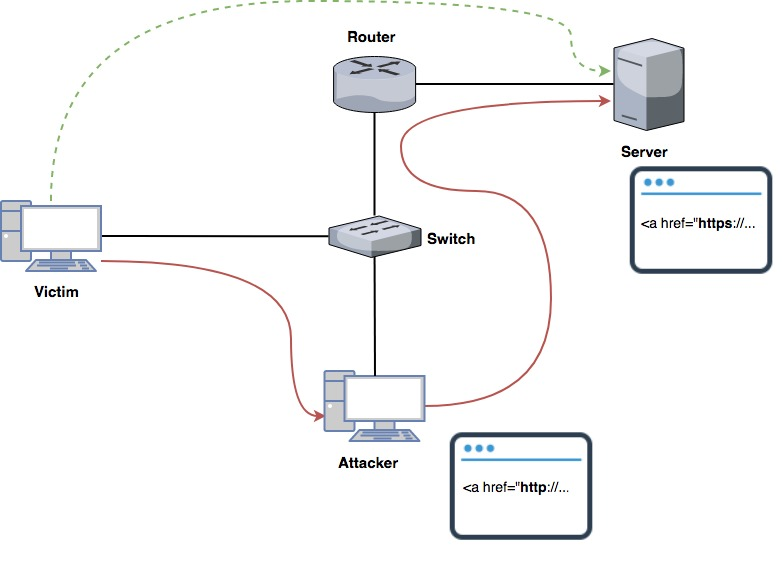
\includegraphics[height=120px]{figures/sslstrip}
      \caption*{SSL Stripping attack diagram}
    \end{figure}
  }
  \only<2>{
  \begin{figure}
    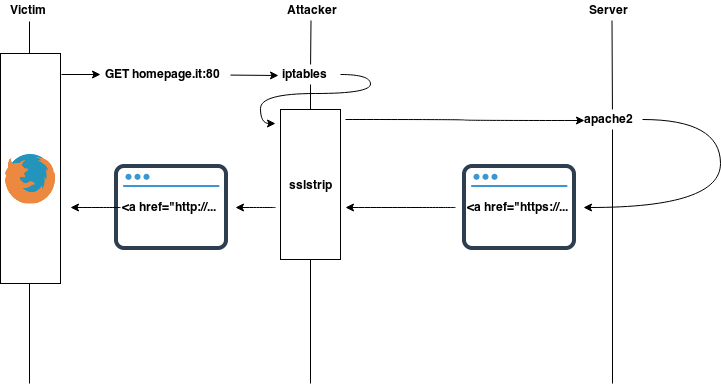
\includegraphics[height=120px]{figures/sslstrip_time}
    \caption*{SSL Stripping attack diagram}
  \end{figure}
  }
\end{frame}

\begin{frame}{SSL Stripping}
  \begin{block}{How it works}
    \begin{itemize}
      \item The URL in the page is sent from the server to SSLstrip
    \end{itemize}
  \end{block}
  \begin{figure}
    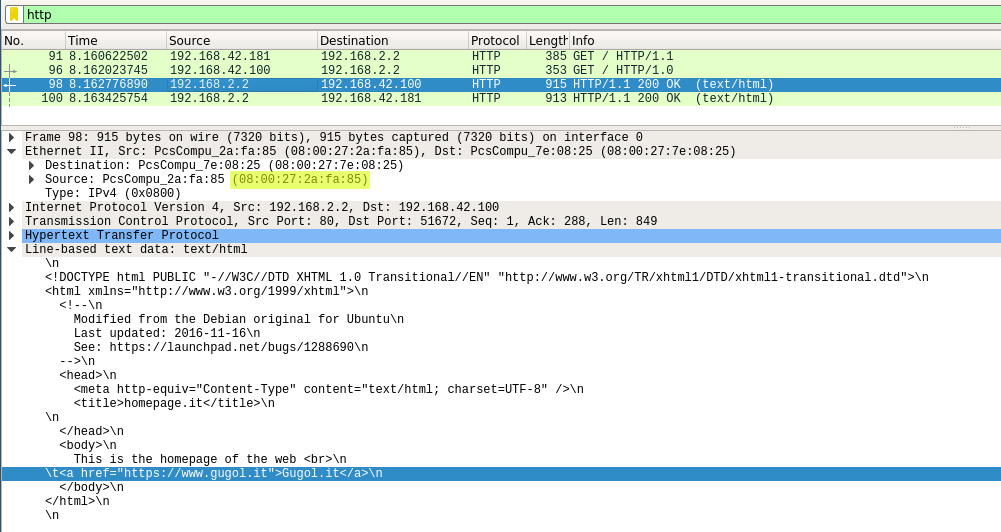
\includegraphics[width=\textwidth]{figures/sslstrip_https}
    \caption*{}
  \end{figure}
\end{frame}

\begin{frame}{SSL Stripping}
  \begin{block}{How it works}
    \begin{itemize}
      \item SSLstrip replaces every \texttt{https://} link with the respective \texttt{http:// one}
    \end{itemize}
  \end{block}
  \begin{figure}
    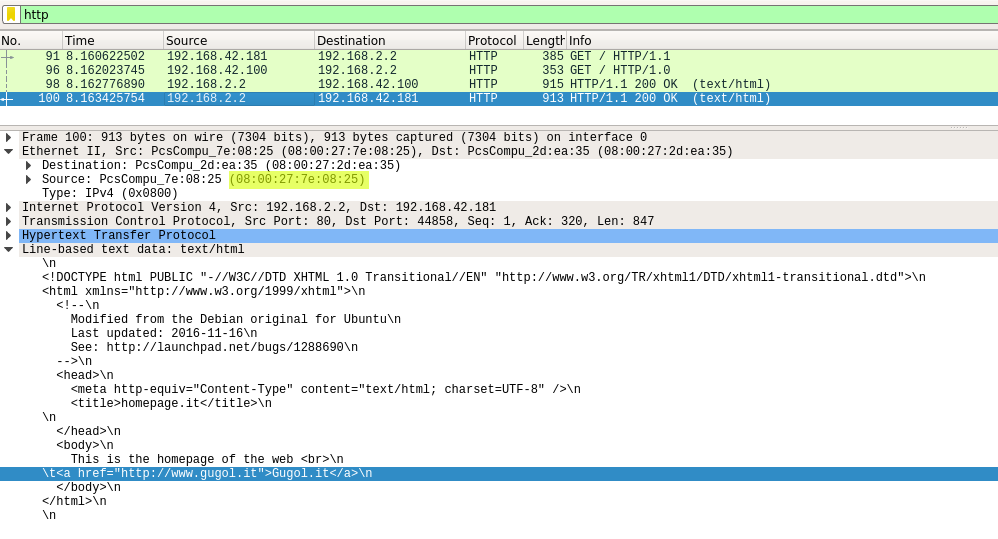
\includegraphics[width=\textwidth]{figures/sslstrip_http}
    \caption*{}
  \end{figure}
\end{frame}

\begin{frame}{SSL Stripping}
  \begin{block}{In practice}
    \begin{itemize}
      \item \texttt{sslstrip} is an HTTP proxy that manipulates the messages to perform the attack
      \item The HTTP traffic flowing through the attacker must be redirected to \texttt{sslstrip}
    \end{itemize}
  \end{block}
  \begin{block}{Usage}
  \texttt{sslstrip -l <port>}
  \end{block}
\end{frame}
\begin{frame}{SSL Stripping}
  \begin{block}{Exercise 2}
    \begin{itemize}
      \item Mount a MitM attack
      \item Setup \texttt{sslstrip} to manipulate the HTTP traffic
      \item Using \texttt{iptables} redirect the traffic from the port 80 to the port that \texttt{sslstrip} is using
      \item Intercept the traffic using Wireshark
      \item Navigate to \texttt{www.homepage.it} and click to the URL
      \item Analyze the behaviour of \texttt{sslstrip}
    \end{itemize}
  \end{block}
  \pause
  \texttt{iptables -t nat -A PREROUTING -p tcp --destination-port <web server port> -j REDIRECT --to-port <sslstrip port>}

\end{frame}
\begin{frame}{SSL Stripping}
  \begin{block}{How to prevent?}
  \pause
  \begin{itemize}
      \item HTTP Strict Transport Security (HSTS) is a web security policy to protect against protocol downgraded attacks
      \item Declaring the HSTS policy, the web server forces a browser to use HTTPS
      \item The HSTS policy is communicated by the server via an HTTPS response header field named \textit{Strict-Transport-Security}
    \end{itemize}
  \end{block}
  \pause
  % \begin{block}{Try it yourself}
  % \begin{itemize}
  %     \item Navigate directly to \texttt{https://www.gugol.it}
  %     \item Try to mount the attack again
  %   \end{itemize}
  % \end{block}
\end{frame}


\begin{frame}{HSTS Bypass}
\only<1>{
  \begin{block}{How it works}
  \begin{itemize}
      \item The HSTS policy is associated with a specific domain name
      \item Changing just by one letter the domain name, the browser will not apply the policy anymore
      \item For example an 'l' (uncapital L) could become an 'I' (capital i)
    \end{itemize}
  \end{block}
  }
  \only<2>{
  \begin{figure}
    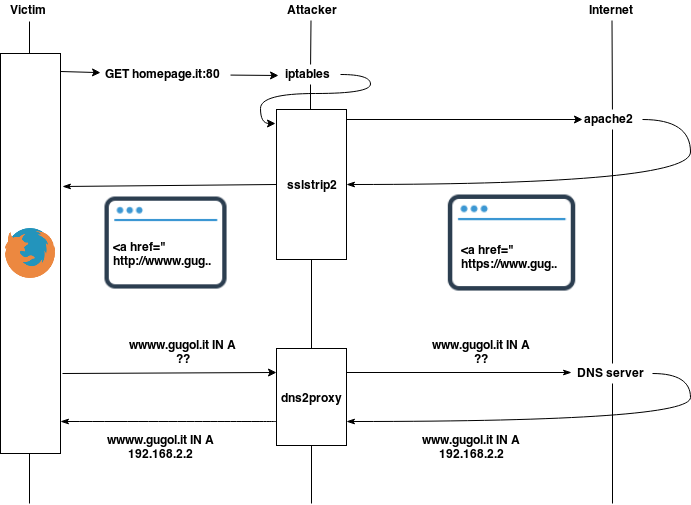
\includegraphics[width=.9\textwidth]{figures/hsts_bypass_time}
    \caption*{}
  \end{figure}
  }
\end{frame}
\begin{frame}{HSTS Bypass}
  \begin{block}{In practice}
  \begin{itemize}
      \item \texttt{sslstrip} can be modified to change the domain name inside the url all the times it strips an HTTPS url
      \item The DNS queries must also be manipulated using \texttt{dns2proxy}
    \end{itemize}
  \end{block}
  \begin{block}{Usage}
  \begin{itemize}
      \item sslstrip2 is in \texttt{Desktop/sslstrip2-exercise/}
      \item It can be executed running \texttt{./sslstrip2 -l <port>}
      \item dns2proxy is in \texttt{Desktop/dns2proxy-exercise/}
      \item It can be executed running \texttt{./dns2proxy}
  \end{itemize}
  \end{block}
\end{frame}
\begin{frame}{HSTS Bypass}
  \begin{block}{Exercise 3}
  \begin{itemize}
      \item Mount a MitM attack
      \item Implement the missing code in \texttt{sslstrip/URLMonitor.py}
      \item Redirect all the traffic in the attacker VM from the port 80 to the port where sslstrip2 is running
      \item Implement the missing code in \texttt{dns2proxy.py}
      \item Verify that dns2proxy is working properly using \texttt{nslookup}
      \item Redirect all the traffic in the attacker VM changing the destination ip
      \item Analyze the behaviour using Wireshark
  \end{itemize}
  \end{block}
  \pause
  \texttt{iptables -t nat -A PREROUTING -p udp --destination-port 53 -i enp0s8 -j DNAT --to <attacker ip>}
\end{frame}
\begin{frame}{HSTS Bypass - sslstrip2 code}
\only<1>{
  \begin{figure}
    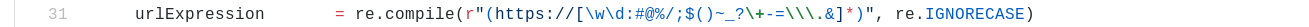
\includegraphics[width=\textwidth]{figures/regexp}
  \end{figure}
  \begin{figure}
    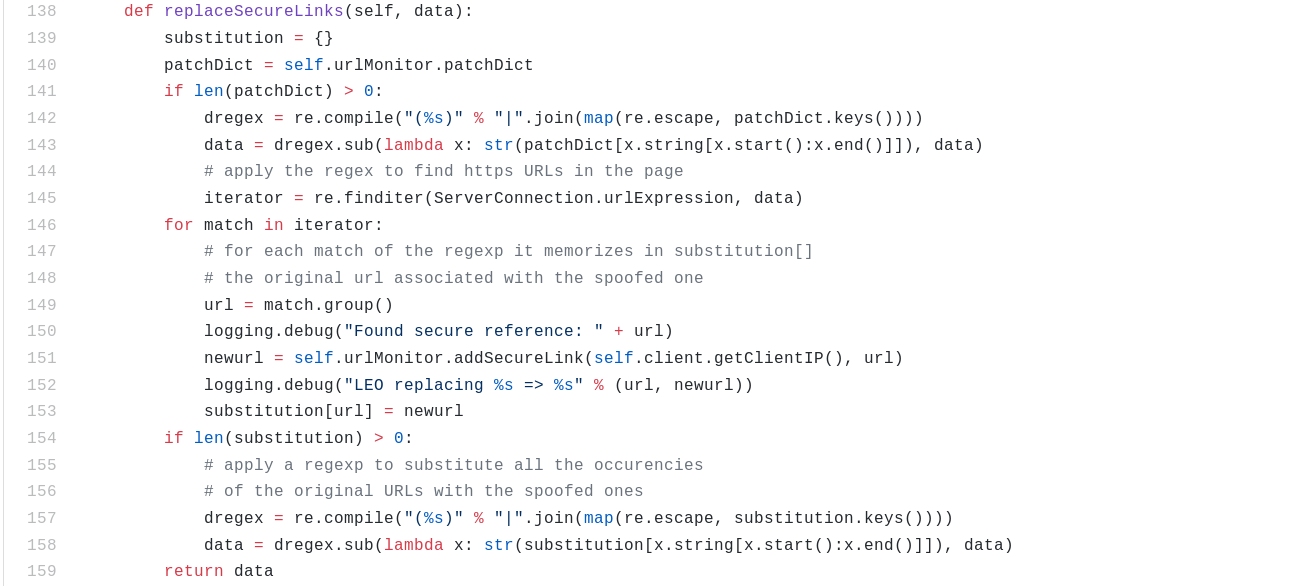
\includegraphics[width=\textwidth]{figures/replace_secure_link}
  \end{figure}
}
\only<2>{
  \begin{figure}
    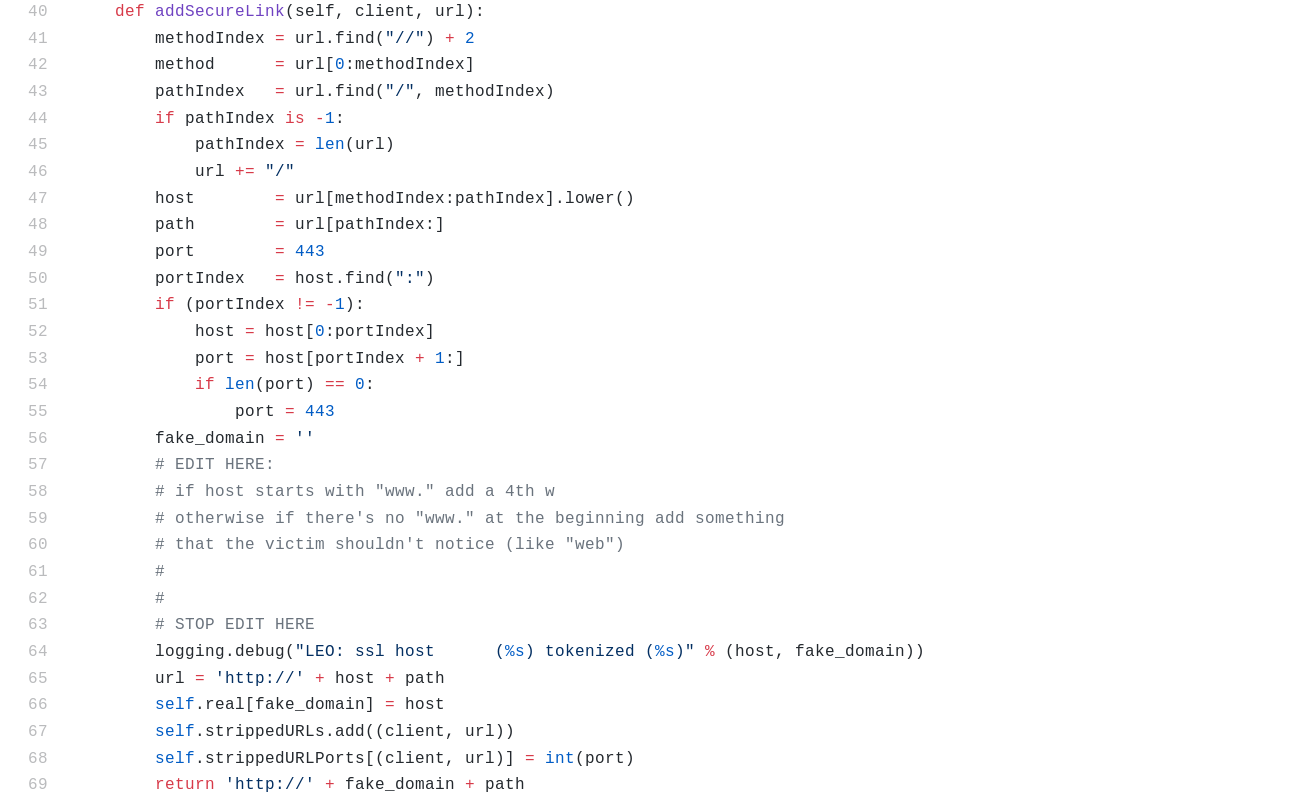
\includegraphics[width=\textwidth]{figures/add_secure_link}
    \caption*{}
  \end{figure}
}
\end{frame}

\begin{frame}{HSTS Bypass - dns2proxy code}
\only<1>{
  \begin{figure}
    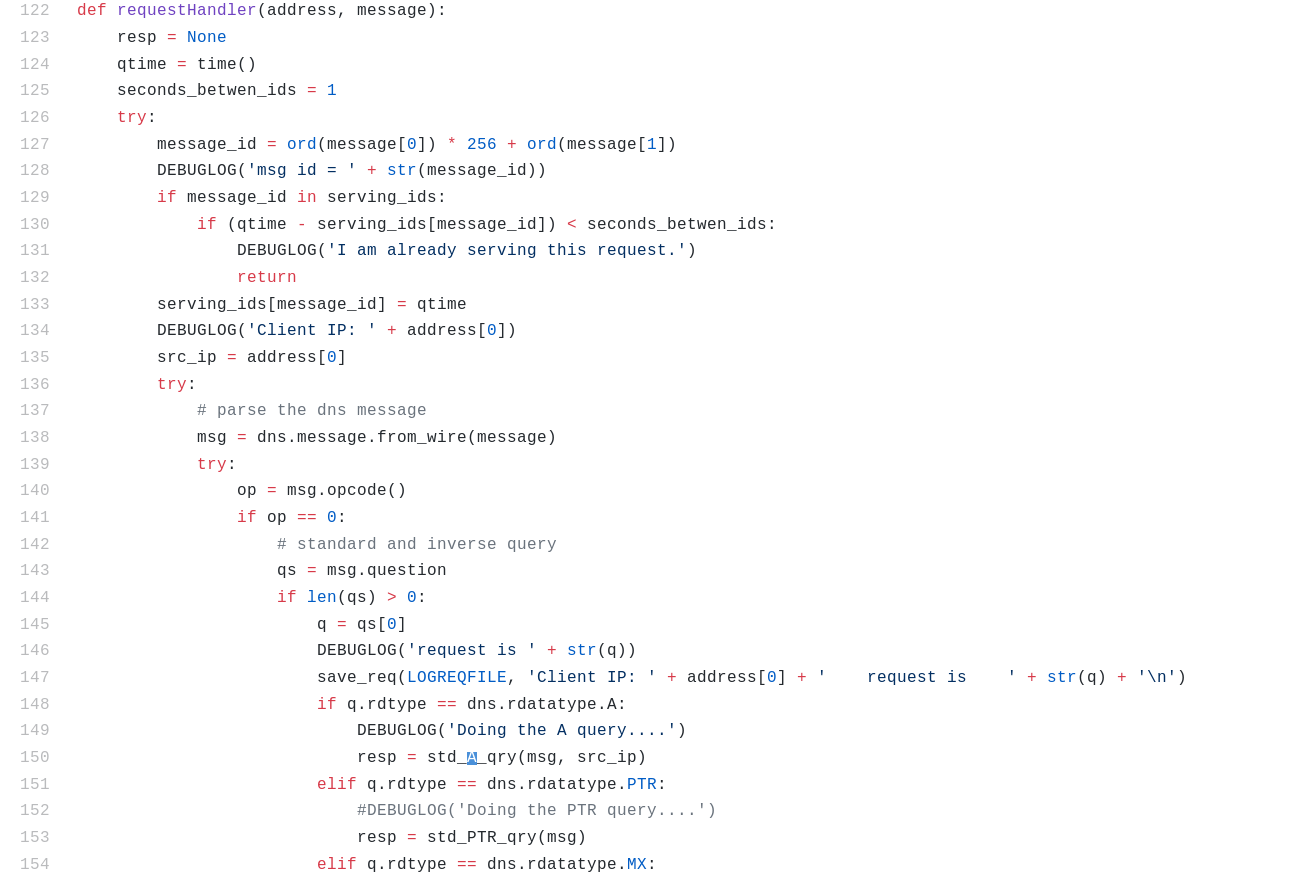
\includegraphics[width=\textwidth]{figures/request_handler}
    \caption*{}
  \end{figure}
}
\only<2>{
  \begin{figure}
    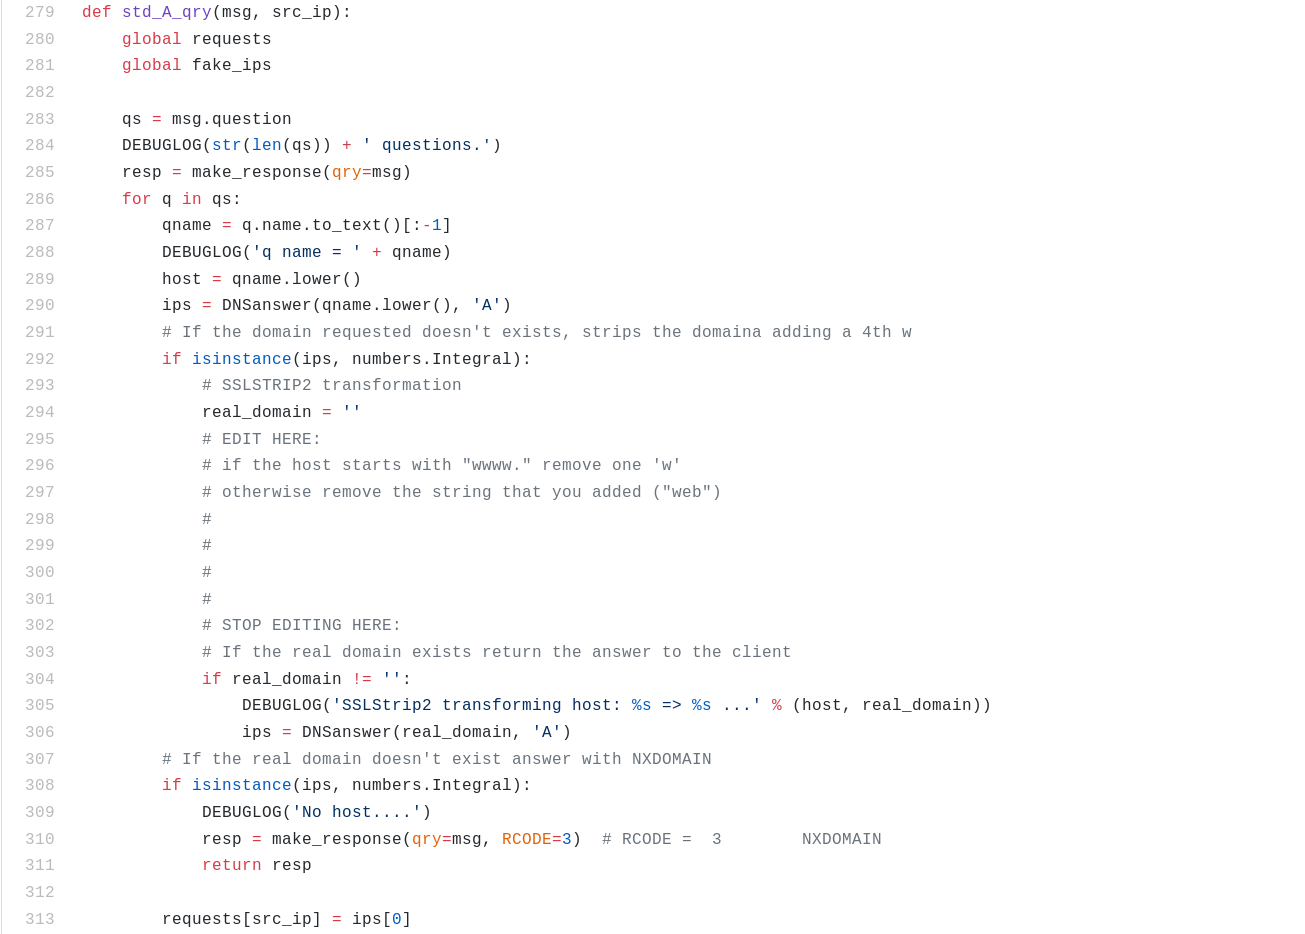
\includegraphics[width=\textwidth]{figures/a_query}
    \caption*{}
  \end{figure}
}
\end{frame}

\begin{frame}{HSTS Bypass}

  \begin{block}{How to prevent?}
    \begin{itemize}
      \pause
      \item The user must always check the correctness of the URL in the address bar
    \end{itemize}
  \end{block}
\end{frame}

\begin{frame}{DNS Spoofing}
  \begin{block}{How it works}
    \begin{itemize}
      \item DNS messages are exchanged in clear using the UDP protocol on port 53
      \item An attacker who is \textit{in the middle} can manipulate the DNS responses
    \end{itemize}
  \end{block}
  \begin{figure}
    \includegraphics[height=100px]{figures/dns-spoof-bad}
    \caption*{Diagram of the attack}
  \end{figure}
\end{frame}
\begin{frame}{DNS Spoofing}
  \begin{block}{In practice}
    \begin{itemize}
      \item \texttt{dnsspoof} forges replies to arbitrary DNS queries on the LAN
    \end{itemize}
  \end{block}
  \begin{block}{Usage}
    \texttt{dnsspoof [-i interface] [-f hostsfile]}
    \begin{block}{}
      The hostfile contains the record associated with the A response\\
      for example:\\
      \texttt{www.google.it  ~~~~192.168.1.1}\\
      \texttt{www.facebook.com   ~192.168.1.1}
    \end{block}
  \end{block}
\end{frame}
\begin{frame}{DNS Spoofing}
  \begin{block}{Exercise}
    \begin{itemize}
      \item There's a malicious webserver running on the attcker VM
      \item Create a proper hostsfile to spoof requests for \texttt{www.gugol.it} pointing to the malicious webserver
      \item Mount a MitM attack
      \item Setup \texttt{dnsspoof} to answer to the DNS query of the victim
      \item Navigate to \texttt{www.gugol.it} to verify that the attacks has succeeded
      \pause
      \item Block the DNS response from the legit server using \texttt{iptables}
    \end{itemize}
  \end{block}
  \pause
  \texttt{iptables -A FORWARD -s <victim ip> -p udp --dport <dns port> -j DROP}
\end{frame}

\begin{frame}{DNS Spoofing}
  \begin{block}{How to prevent?}
  \pause
  \begin{itemize}
    \item Cached responses cannot be spoofed
    \item DNSSec guarantees integrity of the records by using digital signature
  \end{itemize}
  \end{block}
\end{frame}

\begin{frame}{Thank you}
\end{frame}


\end{document}
